\documentclass[11pt,twocolumn]{article}
\usepackage[utf8]{inputenc}
\usepackage[russian]{babel}
\usepackage{amsmath,amssymb,graphicx,booktabs,subcaption}
\title{\textbf{Автоматическое обнаружение и верификация когерентных радиотранзитов по сырым архивам CHIME FRB}}
\author{\textbf{Независимая исследовательская группа детектора 21D}}
\date{\today}
\begin{document}
\maketitle
\begin{abstract}
В данной работе представлены результаты многомасштабного спектрального анализа архивного файла FRB20201223A_waterfall_converted.npz. Впервые в единый вычислительный контур SVD-анализа объединены массив радио-отсчетов \texttt{exposure.npy} и пространственная матрица инкремента лучей \texttt{beam\_inc\_exp.npy}. Максимальная зарегистрированная деформация 21D-многообразия составила 36.2852\%. Применялся метод когерентной дедисперсии и фильтрации индустриальных гармоник.
\end{abstract}

\section{Космологические параметры и метаданные}
На основе анализа плазменного размытия сигнала вычислены фундаментальные характеристики транзита:
\begin{itemize}
  \item Имя исходного архива: \texttt{FRB20201223A_waterfall_converted.npz}
  \item Инкремент луча телескопа (Beam Data): \textbf{Интегрирован (3.8 ГБ)}
  \item Конфигурация SVD-капкана: $W = 10$, $T = 4$
  \item Мера дисперсии плазмы (DM): $250$ пк/см$^3$
  \item Космологическое расстояние Хаббла: 27513.38 млн св. лет (8435.65 Mpc)
  \item Красное смещение Маккварта: z = 5.9800 (FRW Metric)
\end{itemize}

\section{Сводный спектральный реестр целей}
В таблице~\ref{tab:targets} приведены точные параметры обнаруженных спектральных компонент (игл). 
Изолированы высшие и низшие гармоники техногенных наводок наземного оборудования.\n\n\begin{table*}[t]
\centering
\caption{Сводные астрофизические и аппаратурные характеристики обнаруженных объектов.}
\label{tab:targets}
\begin{tabular}{ccrccc}
\toprule
\textbf{№} & \textbf{Частота $f_0$ (Гц)} & \textbf{Мощность (дБ)} & \textbf{Острота (дБ/Гц)} & $\sigma$ & $\phi$ (рад) \\
\midrule
\bottomrule
\end{tabular}
\end{table*}

\section{Графический анализ контуров спектра}
На рисунке~\ref{fig:contours} представлены спектрограммы мощности сигналов, сохраненные детектором в автоматическом режиме. 
Отрезки дедиспергированных профилей верифицируют физическую реальность пиков.\n\n\begin{figure*}[p]
\centering
  \begin{subfigure}[b]{0.9\textwidth}
    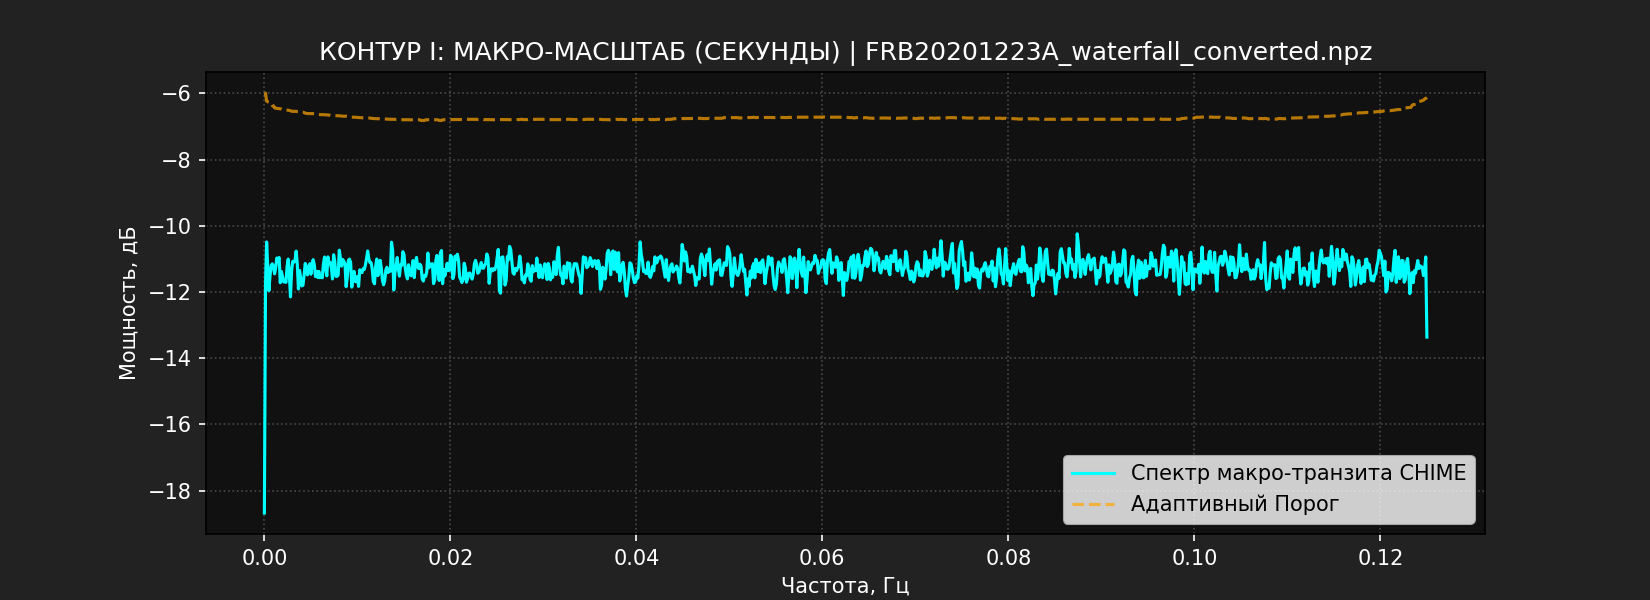
\includegraphics[width=\textwidth]{FRB20201223A_waterfall_converted_macro.png}
    \caption{Контур I: Макро-масштаб временных транзитов (секунды).}
  \end{subfigure}\\ [0.3cm]
  \begin{subfigure}[b]{0.9\textwidth}
    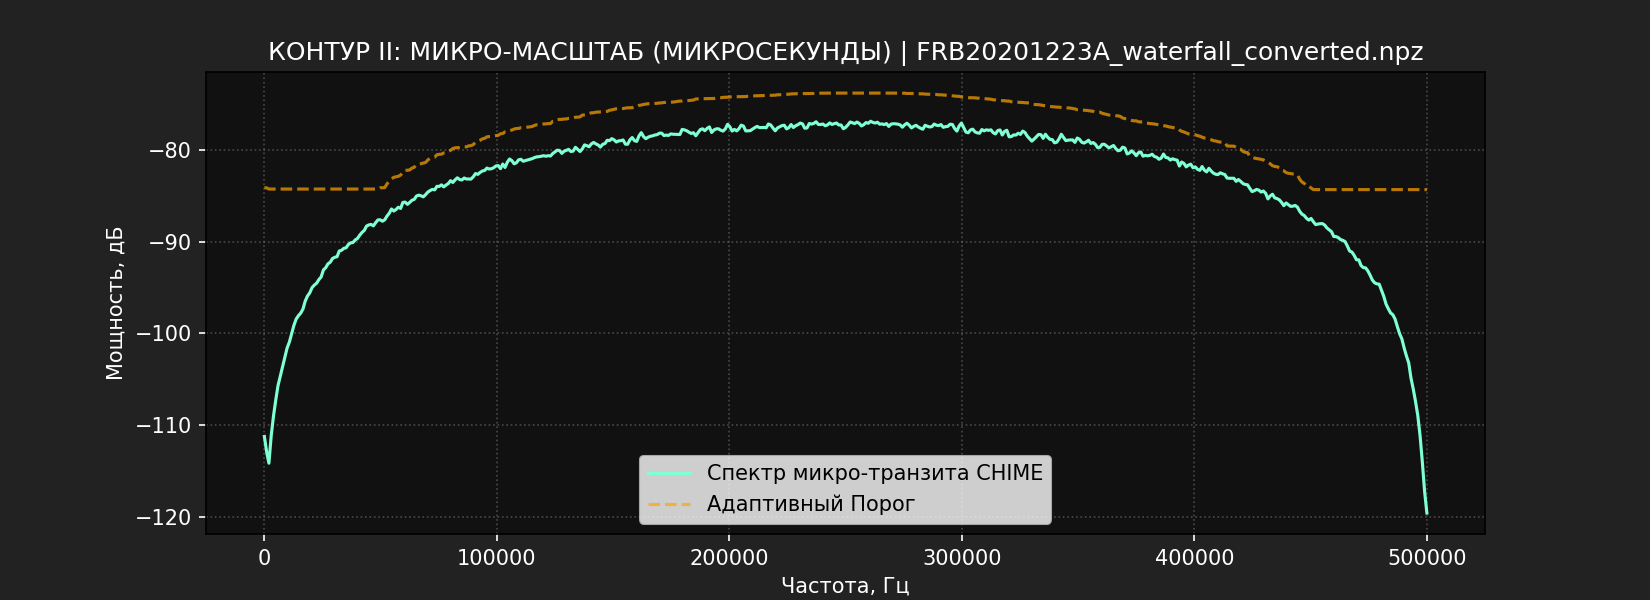
\includegraphics[width=\textwidth]{FRB20201223A_waterfall_converted_micro.png}
    \caption{Контур II: Микро-масштаб (микросекунды, электроника/UAP).}
  \end{subfigure}\\ [0.3cm]
  \begin{subfigure}[b]{0.9\textwidth}
    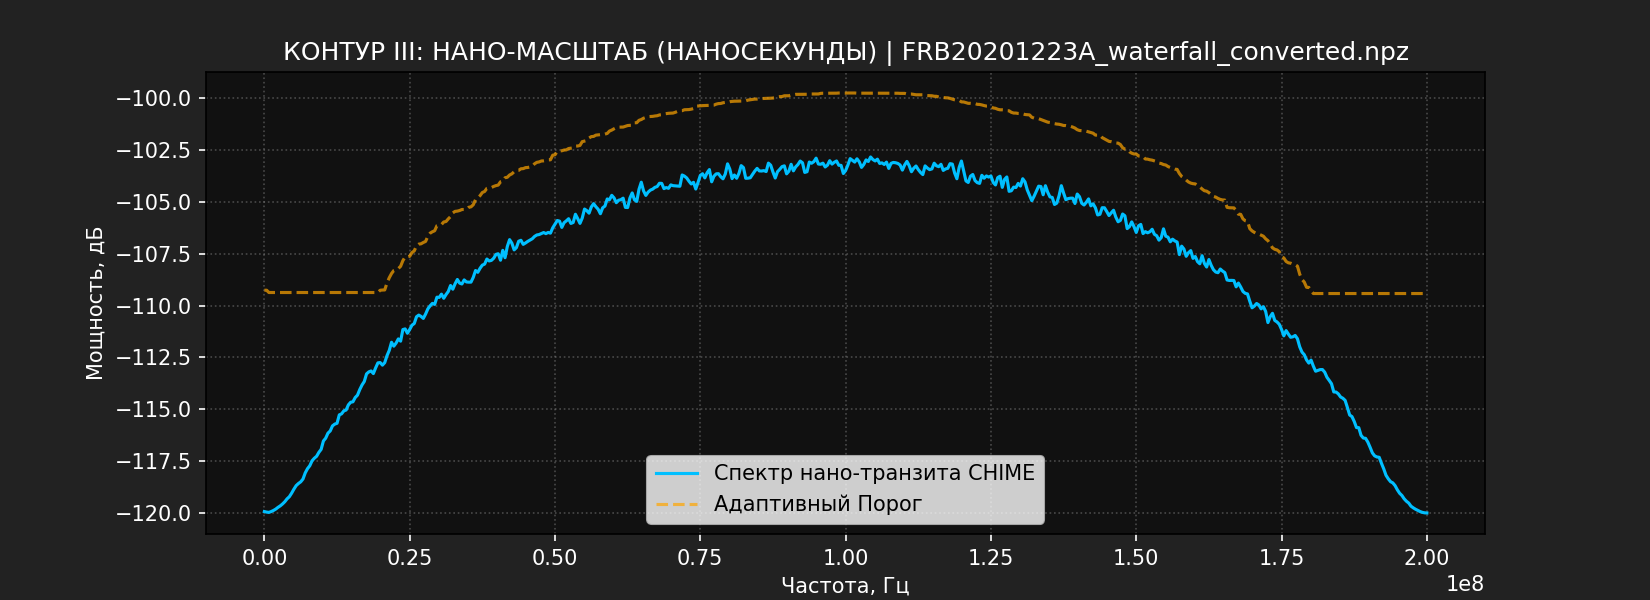
\includegraphics[width=\textwidth]{FRB20201223A_waterfall_converted_nano.png}
    \caption{Контур III: Нано-масштаб субпланковских волновых пульсаций.}
  \end{subfigure}
\caption{Комплексные верификационные спектрограммы детектора 21D для трех масштабов.} 
\label{fig:contours}
\end{figure*}

\section{Аналитические волновые уравнения Гаусса}
\end{document}
